 \documentclass[journal]{IEEEtran}
\interdisplaylinepenalty=2500

\usepackage{array}
\usepackage{graphicx}
\usepackage{epsf}
\usepackage{float}
\usepackage{stfloats}
\usepackage[font=footnotesize]{caption}
\usepackage[font=footnotesize]{subcaption}
\usepackage{cite}
\usepackage{picinpar}
\usepackage{siunitx}

\usepackage{amsmath, nccmath}
\usepackage{url}
\usepackage{flushend}
\usepackage{colortbl}
\usepackage{soul}
\usepackage{multirow}
\usepackage{pifont}
\usepackage{color}
\usepackage{alltt}
\usepackage[hidelinks]{hyperref}
\usepackage{enumerate}
\usepackage{siunitx}
\usepackage{breakurl}
\usepackage{epstopdf}
\usepackage{pbox}


\usepackage{booktabs}
\usepackage{wrapfig}

\graphicspath{{../}}

\usepackage{placeins}
\usepackage{latexsym}
\usepackage{amssymb}
\usepackage{xifthen}
\usepackage{balance}
\usepackage{multicol}
\renewcommand{\arraystretch}{1.2}




\newenvironment{conditions}
  {\par\vspace{\abovedisplayskip}\noindent\begin{tabular}{>{$}l<{$} @{${}-{}$} l}}
  {\end{tabular}\par\vspace{\belowdisplayskip}}


\ifCLASSINFOpdf

\else
 
\fi


\hyphenation{op-tical net-works semi-conduc-tor}


\begin{document}

\title{Analysis and DSP Implementation of Multisampled Digital Control of Electrical Drives}


% make the title area
\maketitle

\begin{abstract}
nothing yet
\end{abstract}

% Note that keywords are not normally used for peerreview papers.
\begin{IEEEkeywords}
nothing yet
\end{IEEEkeywords}


\IEEEpeerreviewmaketitle

\section{Introduction}
\IEEEPARstart{F}{ield} oriented control (FOC) is a well-established strategy for the control of high performance electrical drives \cite{holmes2012}. An essential part of this concept is the inner current control loop \cite{holmes2009}. A prerequisite for the proper operation of the outer control loops is a precise and rapid digital current controller \cite{yepes2014}. In order to achieve the desirable performance of the overall control system high current loop bandwidth is imperative \cite{choi1998}. Robustness at high output frequencies, along with a decoupled d and q axis transient operation is also required ~\cite{choi1998,hoffmann2016,yim2009}. Digital control introduces delays due to the sampling process, execution time and digital pulse width modulation (DPWM) \cite{holmes2009}. These delays limit the achievable bandwidths and motivate the direct discrete-time domain design of high-performance current controllers \cite{bae2003}. These limitations have inspired investigating multisampled PWM control, with purpose of enabling analog-like control bandwidths in digital systems. The multisampling approach relies on acquiring the control variables and updating the modulating waveform multiple times per switching period \cite{corradini_analysis}. The concept of multisampled digital control offers significant reduction of the modulator delays and therefore is a promising solution for breaking the bandwidth limitations \cite{corradini2018}. Besides improvements in dynamic perofrmance, MS-PWM is also reported to have a positive impact on the noise attenuation \cite{petric2020}. 

Synchronous rotating frame (SRF) PI controllers are the most frequently encountered current control concepts since they are simple and successfully cover the majority of the industry requirements ~\cite{rowan1986,bae2003,yepes2014}. With a proper parameter setting procedure, high bandwidths can be achieved ~\cite{yepes2014,holmes2009}. Nevertheless, their transient decoupling capability is rather limited, especially at high speeds \cite{lorenz2000}. On the other hand, model predictive dead-beat current controllers offer very fast transient response but at the cost of considerable performance degradation when parameter mismatch occurs ~\cite{malesani1999,xu2019}. Since saturation and temperature variations are very often encountered in electrical drives, a simple dead-beat approach might lead to insufficient performance. An FPGA implementation of the robust multisampled dead-beat control has been proposed in \cite{rovere2018}. Another promising current control approach is the discrete internal model principle (IMC) design \cite{lorenz2010}. Since no S domain based delay approximations are used, axes cross-coupling is inherently eliminated and high closed loop bandwidths can be achieved ~\cite{commentsHoffmann,vuksa2016}. Despite all of the benefits of feedback averaging, the addition of a moving average filter in feedback path can considerably degrade the performance of the current control loop \cite{vuksa2016}. The IMC concept however, with some enhancements of the controller structure in terms of addition of differential compensator and advanced scheduling scheme, achieves very fast and robust current tracking even with MAF in the feedback path \cite{vuksa2017}. Further improvements in terms of active resistance feedback result in high disturbance rejection capability \cite{vuksa2018}. 

This paper analyzes the use of MS-PWM in discrete IMC based current controller, suitable for implementation on standard DSP platforms. The main goal of the paper is to demonstrate a current control structure, which offers improved dynamic response and high noise suppression compared to the state-of-the-art double update rate solutions. This is achieved without relying on expensive and complicated control platforms, but on a standard industrial DSP. The MS-PWM control strategy is analyzed for three different control loop organizations. The first one uses discrete IMC controller from \cite{vuksa2016}, with a moving average filter (MAF) in the feedback. This case is found to offer slightly improved dynamics compared to standard use of double-update with the same discrete IMC (without filter in feedback) ~\cite{lorenz2010,vuksa2016}, with significant improvement in jitter suppression. Due to added delays introduced by the MAF, the second case adds a derivative action to the controller structure, as in \cite{vuksa2016}. This case is given to demonstrate that MS-PWM can offer even better dynamics than reported in \cite{vuksa2016}. The final case implements MS-PWM based discrete IMC, without any filters in feedback. This case is expected to provide the best dynamics, using discrete IMC without derivative gain. The feedback quality is expected to worsen compared to cases with MAFs, hower, it still retains higher quality compared to double-update \cite{petric2020}. The target is to show that with the multisampling approach delays introduced by feedback averaging can be successfully compensated, by extent determined with the multisampling factor, enabling both robust and error-free feedback acquisition and a high dynamic performance of the current loop.

This paper is organized as follows. Section II addresses discrete time machine model, controller structure and analyzes delays introduced by feedback averaging, calculation and DPWM. The multisampling PWM approach, with an outline of its merits and demerits, is explained in Section III. A DSP implementation of the multisampling algorithm is also presented. Exact controller structures and parameter setting procedures for the three aforementioned cases of interest are derived in Section IV. Effectiveness of the derived analytical model is illustrated via simulated current loop step responses and frequency response analyses. Comparison between performance of the proposed methodology and benchmark controllers is also provided. Experimental results are shown in section V. Conclusions are drawn in section VI, along with a proposal for further studies on the presented topic.
 
\section{Multi-rate control system}

\begin{figure*}[t!]
    \centerline{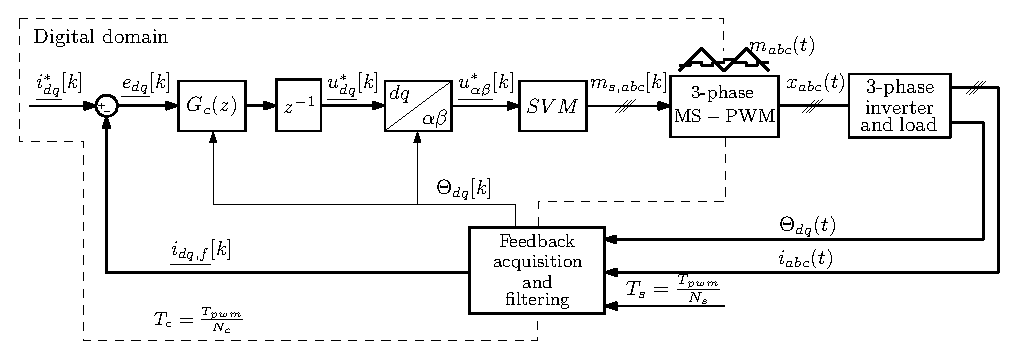
\includegraphics[width=0.95\linewidth]{figures/schematic.eps}}
    \caption{Multisampled control loop of a three-phase inverter. ubaci 1/z da bi bio kompatibilan sa tajming dijagramom}
    \label{fig:MSControl}
\end{figure*}

\subsection{Control system overview and AC machine modeling}
Ovde imas blok dijagram sa strukturom sistema, i small-signal blok dijagram. Nakon toga imas modelovanje masine sa jednacinama...


\subsection{Motivation behind multisampling}
Modern processors enable feature very high computational power, which enables short execution times for control routines. However, switching frequencies of the converter are still hardware limited, and do not go over several tens of kHz for industrial drive applications. This hardware based limitation directly affects the realizable bandwidths of the current control loop, which subsequently limits the speed and position responses as well. Therefore, using multisampled PWM control [] seems to be a logical step forward in the high-performance drive control. 
Using describing function approach, small-signal model of the multisampled PWM with triangular carrier is found to be almost equal to a pure delay of $\frac{T_c}{2}$, where $T_c$ is the modulating waveform update period. Regarding its phase response, the triangular MS-PWM can be well-approximated with the zero-order hold, which is useful for later discrete-time modeling: 

\begin{equation}
G_{DPWM}(s) \approx \frac{1-e^{-sT_c}}{sT_c}, 
\label{eq:DPWM_model}  
\end{equation}
where $s$ is the complex variable of the Laplace transform.

\subsection{Feedback acquisition and $\alpha \beta - dq$ transformation}

\begin{figure}[t!]
    \centerline{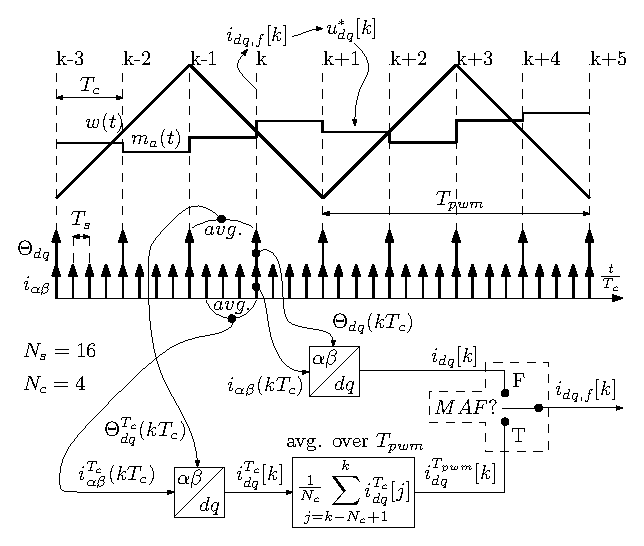
\includegraphics[width=0.95\linewidth]{figures/timing_diagram.eps}}
    \caption{nothing yet}
    \label{fig:timings}
\end{figure}

Ovde onaj blok dijagram od ruzice lep sa transformacijama, pa da se objasni da zapravo koristis i DMA i bla bla .... Prethodno negde na pocetku rada prikazi multi-rate sliku i tu ubaci blok koji se zove feedback acquistion, ulaz su alpha beta struje i ugao, izlaz su dq struje, pa iza toga ide filtar u dq sistemu...

Ovde mozes da kazes: da bi stao ceo kod, ipak ne moze preveliki oversampling faktor. Zbog toga, umesto koriscenja klasicnog koda kao u subsection koji vec, koristi se DMA modul koji sempluje jos n puta brze tako da je ukupan oversampling rate jednak n*N. Nakon tih n odbiraka se zapravo trigeruje interrupt koji je povezan sa N oversamplingom uradi se MAF i decimira se tako da kontrolni kod radi na fc ucestanosti.

Depending on the algorithm complexity, $N_{max} \approx 8$ for $20$ kHz PWM. Since this number cannot be too high, DMA module of the DSP can be used for higher oversampling action that is motivated by noise attenuation and error-free feedback acquisition []. This is performed by triggering sampling each $f_s = nf_c$ and storing results in an DMA array. After $n$ samples are ready, interrupt flag is raised 

Znaci razdvoj ucestanosti:
fpwm - switching
fs - sampling (
fc - control frequency (Nfpwm)



\section{Controller and feedback filter design}

\begin{figure}[t!]
    \centerline{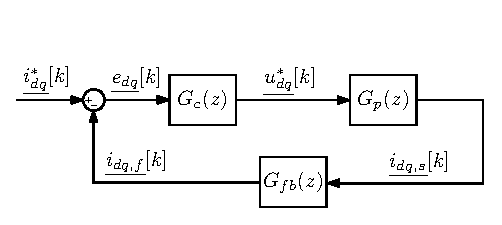
\includegraphics[width=0.95\linewidth]{figures/small_signal.eps}}
    \caption{Small-signal block diagram of the system from Fig. \ref{fig:MSControl} in discrete-time domain.}
    \label{fig:SmallSignal}
\end{figure}

\subsection{Discrete IMC controller}

\subsection{Total time delay in DSP application}
Ovde pricaj o zbirnom kasnjenju, itd....
Mozda nakon price o modelovanju masine...



\section{Simulation results}

\section{Experimental verification}

\section{Conclusion}


\ifCLASSOPTIONcaptionsoff
  \newpage
\fi

\bibliographystyle{IEEEtran}
% argument is your BibTeX string definitions and bibliography database(s)
\bibliography{IEEEabrv,bib/mybibliography.bib}

\end{document}



